\begin{center}
    \textbf{\titlePageWorkType~№\titlePageWorkNumber~\titlePageWorkPart}
\end{center}

\textbf{Тема}: <<\titlePageTopic>>

%\textbf{Цель работы}: 

\begin{center}
    \textbf{Ход работы}:
\end{center}

Написать ассемблерную вставку, реализующую следующую обработку строки: согласно варианту.
Оформить ее в виде отдельной функции.
Реализовать данную обработку строки также в виде функции на С++.
Сравнить быстродействие обоих вариантов.
В отчете отразить выводы.
Для разработки использовать MS Visual Studio.

\textbf{Варианты}:
\begin{enumerate}
    \item[1.] Перевернуть строку.
    \item[2.] Поменять четные символы с нечетными.
    \item[3.] Даны 4 строки. Поменять 1-ю с 3-ей, 2-ю с 4-й.
    \item[4.] Даны 2 строки. Совместить четные символы одной строки с нечентными другой.
    \item[5.] Даны 2 строки. Совместить половину строки 1 с половиной строки 2.
    \item[6.] Нечетные символы заменить на +.
    \item[7.] Совместить 2-е строки. Совпадающие символы заменить на 0.
    \item[8.] Сместить все символы на 1-н вперед циклично.
    \item[9.] Перевернуть две половины строки.
    \item[10.] Сместить все символы на 1-н назад циклично.
    \item[11.] Заменить пробелы на символ табуляции.
    \item[12.] Заменить пробелы на символ табуляции.
    \item[13.] Удалить повторяющиеся пробелы, также пробелы в начале и в конце строки.
\end{enumerate}

Пример функции с ассемблерной вставкой (С++ Visual Studio): 

\begin{lstlisting}[
    name=Пример assembler'ной вставки,
    basicstyle=\ttfamily\scriptsize,
]
    int f()
    {
        __asm
        {
            mov eax, 1
            int 3
        }
        return 0;
    }
\end{lstlisting}

\newpage

\begin{center}
    \textbf{Вариант 6}
\end{center}

\textbf{Условие}:
Нечетные символы заменить на +.

\textbf{Решение}:

\lstinputlisting[
    language=C++,
    basicstyle=\ttfamily\scriptsize,
]
{../../src/option6/src/main.cpp}

\begin{figure}[!htp]
    \centering
    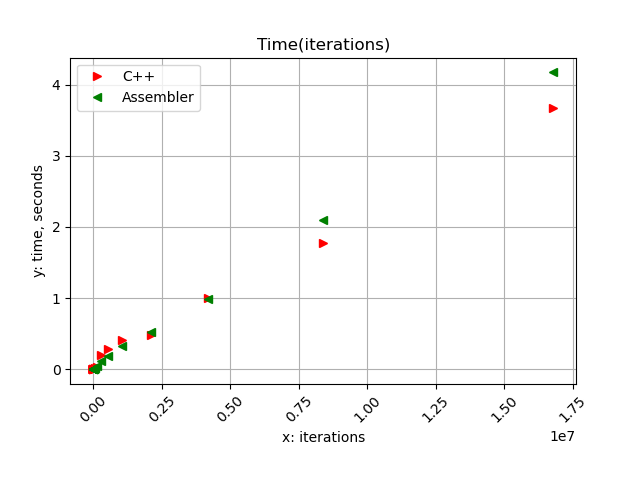
\includegraphics[width=9cm]
    {../_INCLUDES/option6.png}
    \caption{Зависимосте времени от итерации (С++/Assembler)}
\end{figure}

\textbf{Вывод}: ассемблерная ставка медленее C++ на большом количестве итераций вызова.

\newpage

\begin{lstlisting}[
    name=Console log,
    basicstyle=\ttfamily\scriptsize,
]
Test change string on C++
str = "Hello, World!"
str = "H+l+o+ +o+l+!"

Test change string on Assembler
str = "Hello, World!"
str = "H+l+o+ +o+l+!"

           1              0.000000000000        C++
           1              0.000000000000        Assembler
           2              0.000000000000        C++
           2              0.000000000000        Assembler
           4              0.000000000000        C++
           4              0.000000000000        Assembler
           8              0.000000000000        C++
           8              0.000000000000        Assembler
          16              0.000000000000        C++
          16              0.000000000000        Assembler
          32              0.000000000000        C++
          32              0.000000000000        Assembler
          64              0.000000000000        C++
          64              0.000000000000        Assembler
         128              0.000000000000        C++
         128              0.000000000000        Assembler
         256              0.000000000000        C++
         256              0.000000000000        Assembler
         512              0.000000000000        C++
         512              0.000000000000        Assembler
        1024              0.000000000000        C++
        1024              0.001000000000        Assembler
        2048              0.001000000000        C++
        2048              0.001000000000        Assembler
        4096              0.001000000000        C++
        4096              0.000000000000        Assembler
        8192              0.002000000000        C++
        8192              0.001000000000        Assembler
       16384              0.003000000000        C++
       16384              0.005000000000        Assembler
       32768              0.001000000000        C++
       32768              0.004000000000        Assembler
       65536              0.014000000000        C++
       65536              0.017000000000        Assembler
      131072              0.029000000000        C++
      131072              0.050000000000        Assembler
      262144              0.203000000000        C++
      262144              0.112000000000        Assembler
      524288              0.279000000000        C++
      524288              0.180000000000        Assembler
     1048576              0.408000000000        C++
     1048576              0.324000000000        Assembler
     2097152              0.482000000000        C++
     2097152              0.521000000000        Assembler
     4194304              1.008000000000        C++
     4194304              0.987000000000        Assembler
     8388608              1.781000000000        C++
     8388608              2.096000000000        Assembler
    16777216              3.674000000000        C++
    16777216              4.174000000000        Assembler
\end{lstlisting}

\newpage

\paragraph{} Программа, которая рисует график

\lstinputlisting[
   language=Python,
   basicstyle=\ttfamily\scriptsize,
]
{../../src/writeGraph/src/main.py}
